\documentclass[12pt]{article}
\usepackage{geometry}
\usepackage{graphicx}
\usepackage{amsmath}
\usepackage{enumitem}
\usepackage{parskip}
\usepackage{setspace}
\usepackage{float}
\usepackage{relsize}
\usepackage{listings}
\usepackage{fancyvrb}
\usepackage{hyperref}
\usepackage{bookmark}
\usepackage{amsfonts}


\hypersetup{
    colorlinks=true, 
    urlcolor=blue
}

\onehalfspacing
\geometry{letterpaper, portrait, margin=1in}

\newcommand{\qnot}{\scalebox{.8}{$\mathrm{NOT}$}}
\newcommand{\qI}{\scalebox{1}{$\mathrm{I}$}}

\newcommand{\dsum}[2]{\mathlarger{\sum}_{#1}^{#2}}
\newcommand{\bgc}{\begin{center}}
\newcommand{\enc}{\end{center}}
\newcommand{\Lg}{\mathcal{L}}
\newcommand{\norm}[1]{\left\lVert#1\right\rVert}
\newcommand{\colvs}[1]{\begin{bsmallmatrix} #1 \end{bsmallmatrix}}
\newcommand{\colv}[1]{\begin{bmatrix} #1 \end{bmatrix}}
\renewcommand{\arraystretch}{.8}
\newcommand{\state}[1]{\left| #1 \right \rangle}
\newcommand{\tran}{\mathsf{T}}
\newcommand{\sotimes}{\scalebox{.9}{$\otimes$}}
\newcommand{\rarrowtext}[1]{\xrightarrow{\mathrm{#1}}}

\newcommand{\C}[1]{\lstinline{#1}}

\fvset{baselinestretch=1}
\lstset{
  basicstyle=\ttfamily,
  columns=fullflexible,
  keepspaces=true,
}


\begin{document}
\noindent CSCI 4962 \hfill Project Report \\
Siddha Kilaru \\

\bgc
\textbf{Neural Networks as Numeric Solvers}
\enc

\begin{description}
    \item[Introduction] \hfill \\
    The goal of this project is to explore how neural networks can be used to
    approximate solutions to differential equations. The paper ``Physics
    Informed Deep Learning'' by Maziar Raissi, Paris Perdikaris, and George Em
    Karniadakis is the inspiration for this project. The paper introduces the
    concept of physics-informed neural networks and uses it to find solutions
    to nonlinear partial differential equations. In this project, I use the
    methods detailed in the paper but with simpler differential equations.
    Specifically, I focus on first-order and second-order ordinary differential
    equations (ODE), which have analytical solutions. In reality, there is no
    use in approximating a differential equation with an analytical solution;
    however, for the purposes of this project, I want to compute the accuracy
    of the approximated solution. In addition to using the methods outlined in
    the paper, I also experiment with different model hyperparameters and see
    how it affects the runtime and accuracy. Finally, I compare approximate
    solutions derived from neural networks with traditional methods such as
    Euler's and higher-order Runge-Kutta methods.

    \item[Unsupervised Approach] \hfill \\
    Consider the simple differential equation $y' = x$ with initial condition
    $y(0) = 1$. Also, assume we use a neural network to approximate the
    solution in a supervised learning setting. The set of features would be the
    $x$ points, but the set of labels is not immediately obvious. One could say
    the set of labels is a finite set of $y$ points. There are a couple of
    problems, however. First, if the differential equation has no solution,
    then the labels are unattainable. Secondly, if we use real-world, observed
    data, it might be too granular and contain too much noise. As a result, a
    supervised learning model is not completely appropriate for this task. The
    paper mentioned above uses an alternative method that makes use of
    unsupervised learning. The main idea is for the neural networks to learn
    the gradient of the differential equation. Moreover, for a given set of
    labels containing $x$ points, each $x$ point replicates the gradient
    described by the differential equation. In the case of $y' = x$, the
    gradient at each point should be equal to $x$. One way to do this is by
    devising an error function as follows: 
    \bgc 
    $\alpha\Bigl(\dsum{i=0}{n}(\hat{y}_i' - x_i)^2\Bigr)^{1/2} + \beta(\hat{y}_0 - 1)$.
    \enc
    Above, $\alpha$ and $\beta$ are hyperparameters. The first term in the sum
    enforces the ODE constraint, and the second term enforces the initial
    condition. A neural network can use this error function to find an
    approximate solution. Furthermore, the neural network used throughout the
    project is a simple feed forward network with three dense layers.
    Initially, the activation functions were all ReLU; however, since the
    second order differential equations requires second order differentiation,
    I changed the activations to tanh. In the sections below, I experiment with
    different differential equations and their corresponding error functions. 

    \item[Data Exploration and Usage] \hfill \\
    In a standard machine learning project with supervised learning, it would
    be typical to research for quality data sources, analyze/explore the data,
    and perform necessary modifications to get ready for training. However, as
    mentioned in the previous section, this project is focused on unsupervised
    learning. Additionally, I am only focused on exploiting the powerful
    approximation powers of neural networks to fitting analytically defined
    mathematical functions in $\mathbb{R}^n$. Because of this, most of the
    steps mentioned are unnecessary and counterproductive: it does not make
    sense to research for real-world data sets. I need fine control over the
    data I generate because it can drastically affect the neural network's
    performance (numerical methods resort to discretized vectors because it is
    impossible to have continuous variables due to memory and processing
    constraints). 
    
    Not much preprocessing was required to generate data in one dimension
    ($\mathbb{R}^1$). However, generating data for two dimensions
    ($\mathbb{R}^2$) required a non-trivial amount of preprocessing. For
    $\mathbb{R}^1$, it was sufficient to decide on a range $x\in[a, b]$ and the
    number of points $N$ then use \C{torch.linspace(a, b, N)} as needed. In
    contrast, for $\mathbb{R}^2$, the generated vectors need to span a whole
    plane. It is not sufficient to just do $x\in[a, b]$ and $y\in[c, d]$,
    rather we need $A = \{(x, y)~|~x, y \in \mathbb{R};a\leq x \leq b, c \leq y
    \leq d \}$. This requires a lot more computational power: if $N = 500$,
    then the input vector will contain $500^2$ elements. Fortunately, the NumPy
    library has a method \C{numpy.meshgrid} that efficiently implements part of
    this process.

    \item[Approximating First Order ODEs] \hfill \\
    First, let us consider the differential equation $y' = e^x$ with initial
    condition $y(0) = 1$. Trivially, the solution can be analytically
    determined to be $y = e^x$. To approximate the solution, a neural network
    with three hidden layers will be used. One of the hyperparameters for the
    model is the depth of each hidden layer, $d$. The other two hyperparameters
    $\alpha$ and $\beta$ are part of the loss function:
    \bgc 
    $\alpha\Bigl(\dsum{i=0}{n}(\hat{y}_i' -e^{x_i})^2\Bigr)^{1/2} + \beta(\hat{y}_0 - 1)$.
    \enc
    To find the optimal $\beta$, I fix $\alpha = 1$, $d = 20$, and do a search with
    $\beta\in[0, 20]$. The results of the grid search are shown in the plot
    below.\\
    \begin{minipage}{\linewidth}
        \centering
        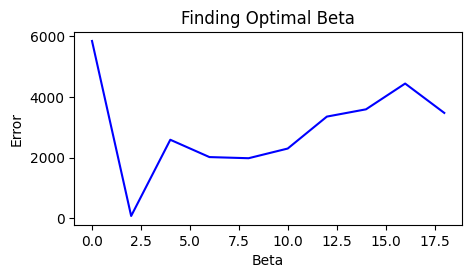
\includegraphics[scale=.5]{images/figure1.png}
    \end{minipage}
    In the plot, the x-axis represents the different $\beta$, and the y-axis is
    the error defined as 
    \bgc 
    $\dfrac{1}{n}\dsum{i=0}{n}(\hat{y}_i - y_i)^2$.
    \enc
    The minimum error occurs when $\beta = 2$, which is the estimated optimal
    value. Next, after training the model, the following results were achieved: \\
    \begin{minipage}{\linewidth}
        \centering
        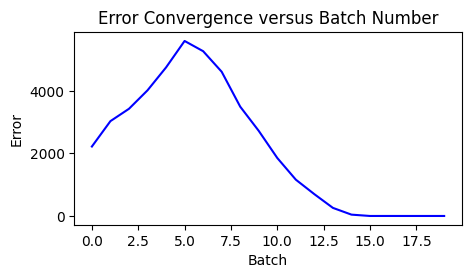
\includegraphics[scale=.5]{images/figure2.png}
    \end{minipage}
    As you can see in the plot above, the error started to decrease rapidly
    just after a few batches. Also, looking at the plots below, the approximate
    solution very closely matches the exact solution. \\
    \begin{minipage}{\linewidth}
        \centering
        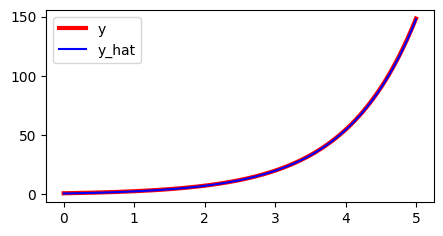
\includegraphics[scale=.5]{images/figure3.png}
        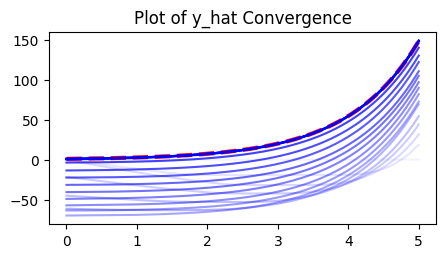
\includegraphics[scale=.5]{images/figure4.png}
    \end{minipage}
    \hfill \\
    \noindent\rule{15.5cm}{.4pt}
    \hfill \\
    Moving on, we now focus on the differential equation $5y' - 4y^2 = 0$ with
    initial condition $y(0) = -8$; the exact solution is $-\frac{40}{32x+5}$.
    The loss function is 
    \bgc 
    $\alpha\Bigl(\dsum{i=0}{n}(5\hat{y}_i' - 4\hat{y}_i^2)^2\Bigr)^{1/2} + \beta(\hat{y}_0 + 8)$.
    \enc
    I find the optimal $\beta = 11$ and $\alpha=1$. Now, I focus on how the
    depth of the neural network affects accuracy and runtime. For $d\in[20,
    500]$, I get the plot below.  \\ 
    \begin{minipage}{\linewidth}
        \centering
        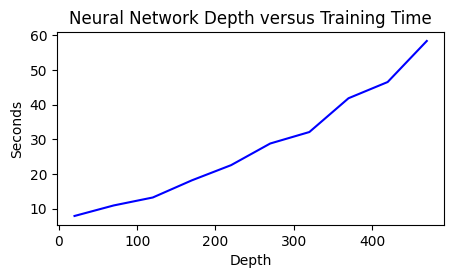
\includegraphics[scale=.5]{images/figure5.png}
        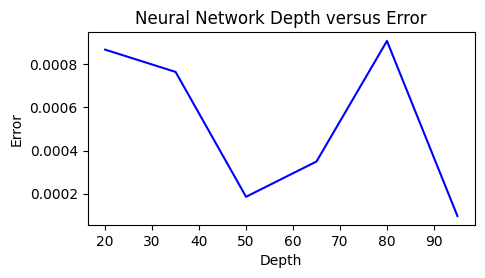
\includegraphics[scale=.5]{images/figure6.png}
    \end{minipage}
    Looking at the plot, there is a clear relationship between depth and
    training time: as the depth increases, the training time increases. The
    relationship appears linear in the plot; however, more investigation is
    needed to determine if that is actually the case. According to the second
    plot, the optimal depth is 95; however, 50 also yields a very low error. If
    we also consider the run time in choosing the optimal depth, then perhaps
    50 is better because of its shorter runtime. Finally, looking at the plots
    below, we can see that the approximate solution is very close to the exact
    solution. \\
    \begin{minipage}{\linewidth}
        \centering
        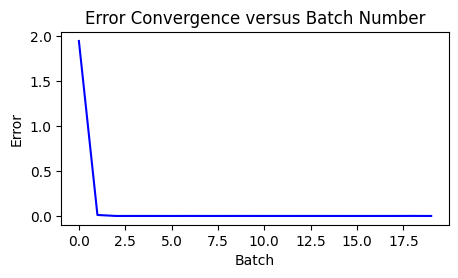
\includegraphics[scale=.5]{images/figure7.png}
        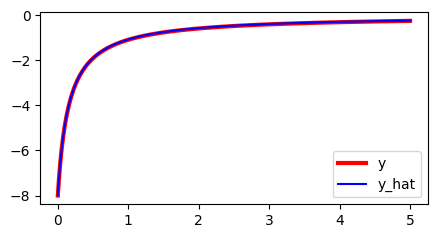
\includegraphics[scale=.5]{images/figure8.png}
    \end{minipage}

    \item[Approximating Second Order ODEs] \hfill \\
    Now, let us experiment with the second-order differential equation $10y''+
    5y = 0$ with initial conditions  $y(0) = 0$ and $y'(0) = 1$; the exact
    solution is $\sqrt{2}\sin(\frac{x}{\sqrt{2}})$. The loss function is 
    \bgc 
    $\alpha\Bigl(\dsum{i=0}{n}(10\hat{y}_i'' + 5\hat{y}_i)^2\Bigr)^{1/2} 
    + \beta(\hat{y}_0)
    + \gamma(\hat{y}_0' - 1)$.
    \enc
    Note that compared to the first order, there is an extra term due to the
    added initial condition. Moving on, I find the optimal $\alpha = 1$, $\beta
    = 1$, and $\gamma = 500$ using the same method. These are the results
    for $x\in[0, 20]$: \\
    \begin{minipage}{\linewidth}
        \centering
        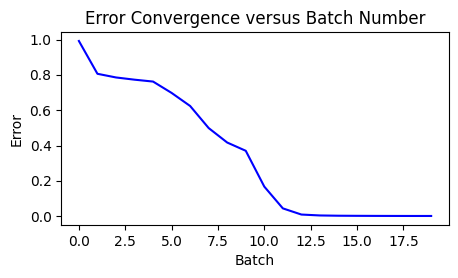
\includegraphics[scale=.5]{images/figure9.png}
    \end{minipage}
    As you can see above, the error decreases significantly toward zero.
    Moreover, looking at the plots below, the approximate solution matches the
    exact solution very closely. \\
    \begin{minipage}{\linewidth}
        \centering
        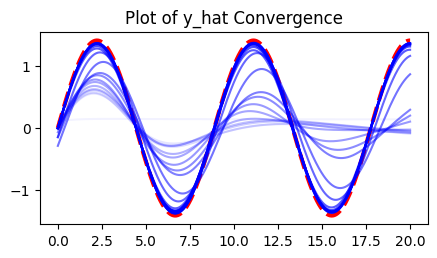
\includegraphics[scale=.5]{images/figure10.png}
        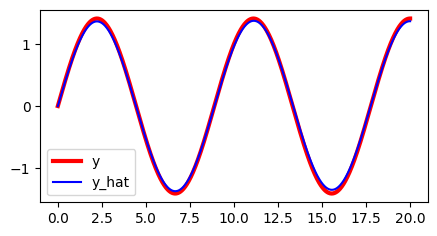
\includegraphics[scale=.5]{images/figure11.png}
    \end{minipage}
    The results shown above are auspicious; however, what does the approximate
    solution look like outside the domain $x\in[0, 20]$ of which the neural
    network was trained on? Looking at the plot below, we can see that
    approximate solution starts to diverge away from the exact solution. This
    kind of behavior is expected because since we only train the neural network
    on a specific range of $x$ values, only those values should have the
    correct gradient. In other words, the model does not prioritize
    generalization at all; instead, the model focuses on approximating as close
    as possible to the desired solution. \\
    \begin{minipage}{\linewidth}
        \centering
        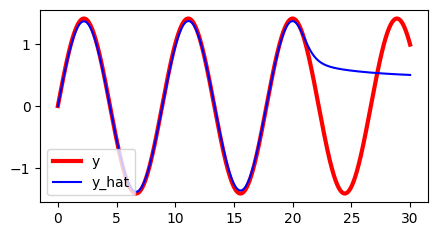
\includegraphics[scale=.5]{images/figure12.png}
    \end{minipage}
    \hfill \\
    \noindent\rule{15.5cm}{.4pt}
    \hfill \\
    Similar to the last differential equation, consider $my'' + by' + ky = 0$.
    In physics, this equation models damped oscillatory behavior, or in other
    words, a damped spring. Let us set $m = 10$, $b = 2$, and $k = 2$. Here the
    mass is $2$, damping constant is $2$, and spring constant is $2$.  Also,
    let the initial conditions be $y(0) = -10$ and $y(0)' = 0$. These
    conditions state that the object starts at position $-10$ with $0$ initial
    velocity. The exact solution to this is 
    \bgc 
    $y(x) = -\dfrac{10}{19} e^{-\frac{x}{10}} (\sqrt{19}\sin(\sqrt{19}x/10) + 19\cos(\sqrt{19}x/10))$,
    \enc
    and the loss function is 
    \bgc 
    $\alpha\Bigl(\dsum{i=0}{n}(10\hat{y}_i'' + 2\hat{y}_i' + 2\hat{y}_i)^2\Bigr)^{1/2} 
    + \beta(\hat{y}_0 + 10)
    + \gamma(\hat{y}_0')$.
    \enc
    Training the neural network with $x\in[0, 55]$ with $50$ points yields the
    results below. \\ 
    \begin{minipage}{\linewidth}
        \centering
        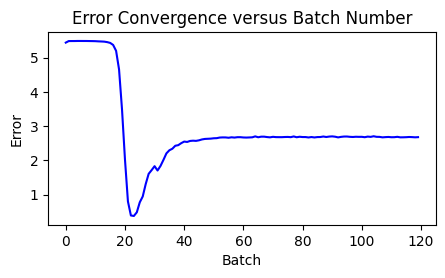
\includegraphics[scale=.5]{images/figure13.png}
        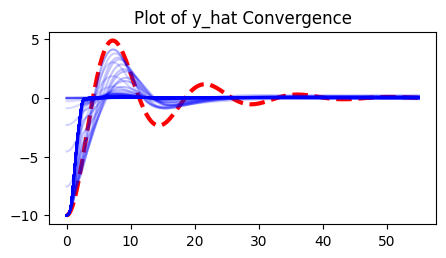
\includegraphics[scale=.5]{images/figure14.png}
    \end{minipage}
    Interestingly, the error rapidly decreases and then starts to increase.
    This is also represented in the second plot, where it first starts to fit
    properly, then starts reverting to a worse approximation. I theorize this
    is due to the fact that 50 points in the range of 0 to 55 are not enough.
    The fewer points cause a single point to appease contrasting gradients.
    Below are the results for the neural network trained with $x\in[0, 55]$
    with $300$ points. \\
    \begin{minipage}{\linewidth}
        \centering
        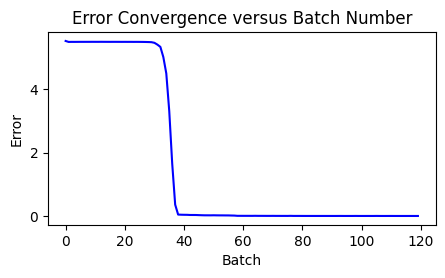
\includegraphics[scale=.5]{images/figure15.png}
        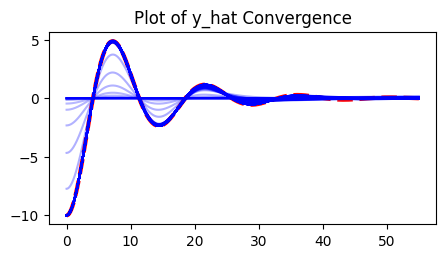
\includegraphics[scale=.5]{images/figure16.png}
    \end{minipage}
    Now, the error function is monotonically decreasing, and the approximate
    solution is very close to the exact solution. Another interesting thing
    about this solution, in particular, is that it decays, or the derivative
    flattens as $x$ increases. A consequence of this is that, unlike the
    previous equation, where the approximate solution deviates away from the
    exact solution, the approximate solution will continue to follow the exact
    solution. This can be seen in the plot below. The network was only trained
    for $x\in[0, 50]$, but the plot is for $x\in[0, 150]$. \\
    \begin{minipage}{\linewidth}
        \centering
        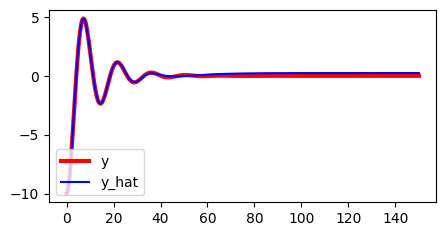
\includegraphics[scale=.5]{images/figure17.png}
    \end{minipage}
    \item[Comparison to Traditional Methods] \hfill \\
    Euler's Method is one of the most popular and simplest methods for
    numerically solving differential equations. One important difference
    between Euler's Method and any finite difference method for solving
    differential equations are that they are iterative. Moreover, if the
    initial condition is at $x=0$, and you desire a solution at $x=100$, then
    you must iteratively compute the solution. So, if the spacing between each
    point is $\kappa$, you must do $\frac{100}{\kappa}$ computations. This can be
    costly because $\kappa$ must be very small to approximate the solution
    accurately. In contrast, with a neural network, any point within the
    trained bounds can be instantly computed with a single feed-forward
    computation. Yes, the neural network requires training time which is
    arguably more costly; further analysis should be done to understand the
    tradeoff between the two methods.

    Below are plots comparing Euler's Method to a neural network's approximate
    for a different number of points $N$. I use the differential equation $5y'
    - 4y^2 = 0$ with initial condition $y(0) = -8$. \\
    \begin{minipage}{\linewidth}
        \centering
        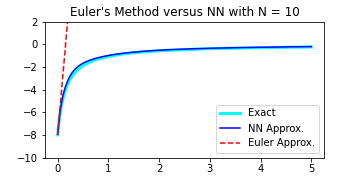
\includegraphics[scale=.5]{images/euler10.png}
        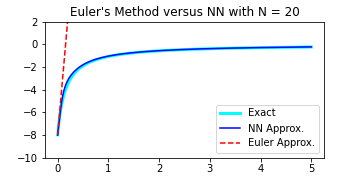
\includegraphics[scale=.5]{images/euler20.png}
        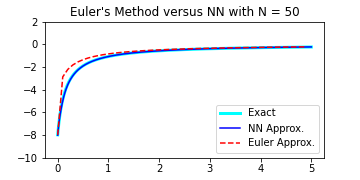
\includegraphics[scale=.5]{images/euler50.png}
        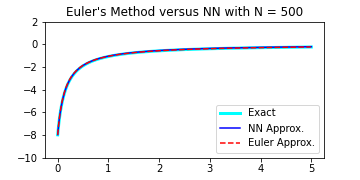
\includegraphics[scale=.5]{images/euler500.png}
    \end{minipage}
    Looking at the plots with $N = 10$ and $N = 20$, the solution created by
    Euler's Method ended up being highly unstable and increasing towards
    infinity. However, with $N = 50$ and $N = 500$, the solution was a fairly
    good fit. The neural network approximation was stable for all $N$ and got
    better as $N$ increased. Even with $N = 10$, the neural network
    approximation was fairly accurate. 
    \hfill \\
    \noindent\rule{15.5cm}{.4pt}
    \hfill \\
    The next traditional method I would like to compare neural networks against
    is RK4. Compared to Euler's Method, RK4 is a lot more robust (much more
    stable) and better at approximating. However, it requires several more
    function evaluations compared to Euler's Method. Below are the plots
    comparing RK4 to a neural network using the same differential equation as
    above. \\
    \begin{minipage}{\linewidth}
        \centering
        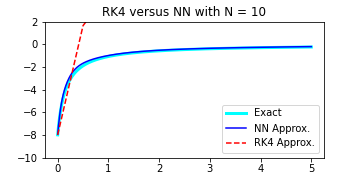
\includegraphics[scale=.5]{images/rk10.png}
        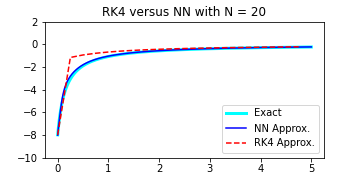
\includegraphics[scale=.5]{images/rk20.png}
        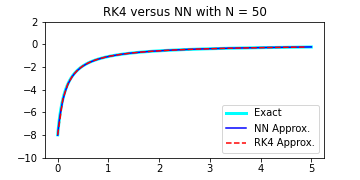
\includegraphics[scale=.5]{images/rk50.png}
        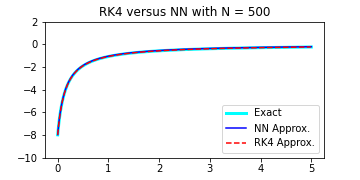
\includegraphics[scale=.5]{images/rk500.png}
    \end{minipage}
    At $N=10$, RK4 is unstable and tends toward infinity. However, at $N=20$,
    unlike Euler's Method, it approximates the solution. At $N=50$ and $N=500$,
    RK4 is spot on. Comparing this to the neural network, we can see that the
    neural network only outperformed with $N=10$ and $N=20$.
    \item[Comparison of Activation Functions] \hfill \\ 
    As mentioned previously, any linear activation function or activation
    function without a second derivative is not sufficient for approximating
    higher order differential equations. The activation function used for all
    the experiments above were tanh, but in this section, I use the SiLU
    activation function: $x * \sigma(x)$. SiLU (swish function) is closely
    related to ReLU, but does allow for approximating second-order differential
    equations. Below is a visual comparison between the different activation
    functions: \\
    \begin{minipage}{\linewidth}
        \centering
        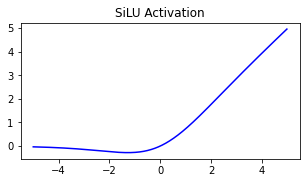
\includegraphics[scale=.45]{images/silu.png}
        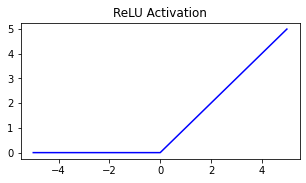
\includegraphics[scale=.45]{images/relu.png}
        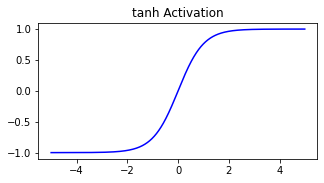
\includegraphics[scale=.45]{images/tanh.png}
    \end{minipage}
    The main problem with using tanh as an activation function is the vanishing
    gradient problem and the usual solution is to use the ReLU activation
    instead. However, as stated above, that will not work, so instead, I used
    SiLU. Below is the error convergence of the same spring damper differential
    equation used above: \\
    \begin{minipage}{\linewidth}
        \centering
        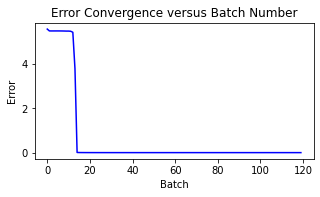
\includegraphics[scale=.5]{images/2ndsiluconv.png}
        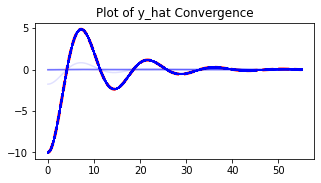
\includegraphics[scale=.5]{images/2ndsilufn.png}
    \end{minipage}
    As you can see, the error dropped to zero just before 20 batches using
    SiLU, but it took about 40 batches using tanh. Additionally, the
    approximated solution matches the exact solution much more closely.

    \item[Approximating a Solution to the Heat Equation] \hfill \\
    The heat equation in one dimension is 
    \bgc 
    $\dfrac{\partial u}{\partial t} = \kappa \dfrac{\partial^2 u}{\partial x^2}$.
    \enc
    The boundary conditions will be 
    \bgc 
    $u(a, t) = 0$ and $u(b, t) = 0$,
    \enc
    and the initial condition is 
    \bgc 
    $u(x, 0) = f(x)$.
    \enc 
    I set the initial distribution for the heat to be $f(x) = 6\sin(x\pi/b)$
    and set $a = 0$, $b = 1$, and $\kappa = 1$. The exact solution is $u(x, t)
    = 6\sin(x\pi)e^{-t\pi^2}$. The loss function is 
    \bgc
    \scalebox{.8}{
    $\alpha\Biggl[\dsum{i=0}{n}\Biggl(\dfrac{\partial \hat{u}_i}{\partial t_i} - \dfrac{\partial^2 \hat{u}_i}{\partial x_i^2}\Biggr)^2\Biggr]^{1/2} 
    + \beta\Biggl(\dsum{i=0}{n}(\hat{u(x_i, 0)} - f(x_i))^2\Biggr)^{1/2}
    + \kappa\Biggl(\dsum{i=0}{n}\hat{u(0, t_i)}^2\Biggr)^{1/2}
    + \gamma\Biggl(\dsum{i=0}{n}\hat{u(1, t_i)}^2\Biggr)^{1/2}$}.
    \enc
    Through experimentation I found the optimal hyperparameters to be $\alpha =
    1, \beta = 250, \kappa = 60$, and $\gamma = 60$. Below is the error
    convergence for $\hat{u(x, 1)}$ over 500 batches. \\
    \begin{minipage}{\linewidth}
        \centering
        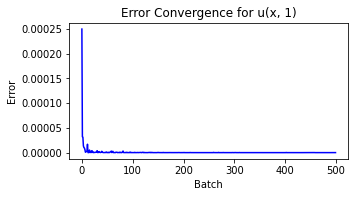
\includegraphics[scale=.5]{images/figure20.png}
    \end{minipage}
    As shown by the plot, the error immediately drops after just a few batches
    and continues to decrease slowly. Training a two-dimensional function took
    much more time than a one-dimensional function. If $n$ training points were
    used in a one-dimensional setting, then comparably, $n^2$ points must be
    used to capture all pairwise relationships. Moreover, on my setup, the
    training times for $n=50$ in the one-dimensional setting was about the same
    as $n=10$ in the two-dimensional setting. 
    
    The plots below are the final results produced by the trained neural
    network: \\
    \begin{minipage}{\linewidth}
        \centering
        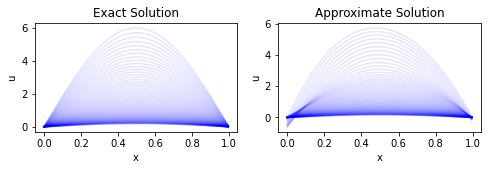
\includegraphics[scale=.5]{images/figure18.png}
        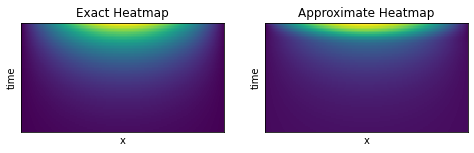
\includegraphics[scale=.5]{images/figure19.png}
    \end{minipage}
    As you can see, the neural network approximates the solution fairly well.
    The two plots on top (the exact and approximate solution) represent the
    plots of $u(x, t)$, where the lighter lines have a $t$ closer to 0. For the
    heatmaps on the bottom, a darker shade is cooler, and the time increases in
    the downward direction of the $y$-axis.

    \item[Conclusion] \hfill \\ 
    The results of my project illustrate that neural networks could be a viable
    approach to approximating differential equations. However, there are
    specific problems with neural networks and the unsupervised approach.
    First, in one of the sections above, I showed that the approximated
    solution becomes unreliable when the inputs used are outside the training
    boundaries. This is a significant drawback in simulating events when there
    is no clear upper bound. Though one possible exception to this is the
    spring damper equation with a decaying solution. Second, training times can
    be very long and not worth using over alternative methods. However, when
    compared to traditional methods, the neural network could approximate with
    fewer points hinting at lower runtimes. Still, more advanced numerical
    methods , such as the RK4 quickly caught up. In conclusion, neural networks
    are dope, but for now, I'd stick to the tried and tested and do more
    research on neural network solvers. 

    \item[Notebook] \hfill \\
    The jupyter notebook for this project can be accessed here: \\
    \url{https://github.com/siddha20/CSCI4962/blob/master/Project/project.ipynb}.
\end{description}


\end{document}